\documentclass{article}

% if you need to pass options to natbib, use, e.g.:
%     \PassOptionsToPackage{numbers, compress}{natbib}
% before loading neurips_2019

% ready for submission
% \usepackage{neurips_2019}

% to compile a preprint version, e.g., for submission to arXiv, add add the
% [preprint] option:
    % \usepackage[preprint]{neurips_2019}

% to compile a camera-ready version, add the [final] option, e.g.:
\usepackage[final]{neurips}

% to avoid loading the natbib package, add option nonatbib:
    % \usepackage[nonatbib]{neurips_2019}
\usepackage{multicol}
\usepackage{float}
\usepackage[center]{caption}

\usepackage[utf8]{inputenc} % allow utf-8 input
\usepackage[T1]{fontenc}    % use 8-bit T1 fonts
\usepackage{hyperref}       % hyperlinks
\usepackage{url}            % simple URL typesetting
\usepackage{booktabs}       % professional-quality tables
\usepackage{amsfonts}       % blackboard math symbols
\usepackage{nicefrac}       % compact symbols for 1/2, etc.
\usepackage{microtype}      % microtypography
\usepackage{graphicx}
\usepackage{amsmath}
\usepackage{xepersian}

\settextfont{XB Yas.ttf}

\title{تکلیف شماره 4
 - 
 \lr{Coordinated Attack, Randomized Version}}


% The \author macro works with any number of authors. There are two commands
% used to separate the names and addresses of multiple authors: \And and \AND.
%
% Using \And between authors leaves it to LaTeX to determine where to break the
% lines. Using \AND forces a line break at that point. So, if LaTeX puts 3 of 4
% authors names on the first line, and the last on the second line, try using
% \AND instead of \And before the third author name.

\author{%
  امیرحسین مهدی‌نژاد\\
  شماره دانشجویی 810800058\\
  \texttt{mahdinejad@ut.ac.ir} \\
  % examples of more authors
  % \And
  % Coauthor \\
  % Affiliation \\
  % \texttt{email} \\
  % \AND
  % Coauthor \\
  % Affiliation \\
  % Address \\
  % \texttt{email} \\
}

% create title (includes both anonymized and non-anonymized versions)
% \providecommand{\@makepertitle}{}
% \newcommand{\makepertitle}{%
%   \vbox{%
%     \hsize\textwidth
%     \linewidth\hsize
%     \vskip 0.1in
%     \toptitlebar
%     \centering
%     {\LARGE\bf \@title\par}
%     \bottomtitlebar
%       \def\And{%
%         \end{tabular}\hfil\linebreak[0]\hfil%
%         \begin{tabular}[t]{c}\bf\rule{\z@}{24\p@}\ignorespaces%
%       }
%       \def\AND{%
%         \end{tabular}\hfil\linebreak[4]\hfil%
%         \begin{tabular}[t]{c}\bf\rule{\z@}{24\p@}\ignorespaces%
%       }
%       \begin{tabular}[t]{c}\bf\rule{\z@}{24\p@}\@author\end{tabular}%
%     \vskip 0.3in \@minus 0.1in
%   }
% }

\begin{document}


\begin{minipage}{0.1\textwidth}% adapt widths of minipages to your needs

\includegraphics[width=1.1cm]{Photos/UT_logo.png}
\end{minipage}%
\hfill%
\begin{minipage}{0.9\textwidth}\raggedleft
دانشکده فنی، دانشگاه تهران\\
سیستم‌های توزیع شده - 
آذر
ماه 1400\\
\end{minipage}
% \end{}

\makepertitle

% ----------------------------------------------------------------------

% \begin{abstract}
%  این بخش از یک پاراگراف تشکیل شده است که توضیحاتی کلی در مورد مساله و راه حل شما ارائه می‌دهد.
% \end{abstract}
\begin{multicols}{2}
مدل مسئله مطابق توضیحات کلاس و متن کتاب
\lr{lynch}:\\
در اینجا 
\lr{n}
نود در گراف کامل بدون جهت داریم که هر نود از توپولوژی خبر دارد و نظر اولیه‌ی آن صفر یا یک است.
\begin{figure}[H]
    \centering
    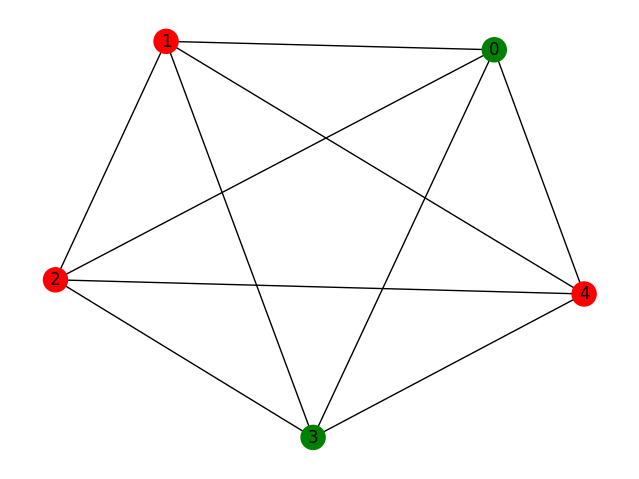
\includegraphics[width=0.95\linewidth]{Photos/HW4/graph.png}
    \caption{
    در اینجا نودهای ۱ و ۲ و ۴ نظرشان صفر (قرمز) و باقی نودها نظرشان یک (سبز) است. انتظار داریم تصمیم نهایی صفر باشد.
    }
    \label{fig:my_label}
\end{figure}
با شبیه‌سازی مسئله، شرایط تصمیم‌گیری را بررسی می‌کنیم:
\begin{itemize}
    \item \lr{Agreement}
    :نباید دو پروسه روی مقادیر مختلف به نتیجه برسند.
    \item \lr{Validity}
    :اگر همه با صفر شروع کردند، نتیجه‌ی نهایی الزاما صفر باشد و اگر همه با یک شروع کردند و پیامی گم نشد، نتیجه‌ی نهایی یک باشد.
    \item \lr{Termination}
    :بالاخره یک جایی همه‌ی نودها به تصمیم برسند.
\end{itemize}
عملا با توجه به اینکه امکان بروز خطا وجود دارد، هیچ راه‌حل قطعی برای مسئله‌ی 
\lr{Consensus}
نداریم و سراغ روش
\lr{Randomized}
می‌رویم.
\section*{توضیحات کد}
فایل
\texttt{random-attack.py}
ضمیمه‌ی این گزارش شده است که بخش‌های اصلی آن را بررسی می‌کنیم:
\begin{figure}[H]
    \centering
    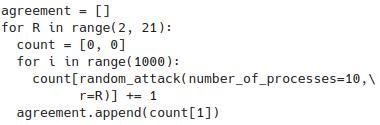
\includegraphics[width=0.99\linewidth]{Photos/HW4/main.png}
    \caption{
    در اینجا ۱۰۰۰ بار تابع حمله‌ی رندوم را به ازای
    \lr{r}
    های مختلف اجرا می‌کنیم تا ببینیم در چند مورد از آن‌ها شرط
    \lr{Agreement}
    برقرار است.
    }
    \label{fig:my_label}
\end{figure}
مطابق شکل، تعداد پروسه‌ها ۱۰ فرض شده و در اندیس صفر از آرایه‌ی
\lr{count}
تعداد دفعاتی که پروسه‌ها بر روی صفر و در اندیس یک، تعداد دفعاتی که بر روی یک توافق کردند نگهداری می‌شود.
\begin{figure}[H]
    \centering
    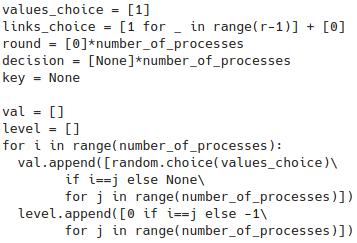
\includegraphics[width=0.95\linewidth]{Photos/HW4/init.png}
    \caption{
    خطوط اولیه‌ی تابع
    \texttt{random\_attack}
    }
    \label{fig:my_label}
\end{figure}
بر اساس شبه‌کد کتاب و با توجه به شکل بالا، گزینه‌ی ممکن برای
\lr{value}
تنها یک در نظر گرفته شده است یعنی می‌خواهیم تمام پروسه‌ها با ۱ شروع کنند و به همین دلیل در شکل قبلی دیدیم که آرایه‌ی
\lr{agreement}
با مقادیر
\lr{count[1]}
پر شد.\\
همچنین احتمال خرابی لینک‌ها در خط بعدی برابر با
$\dfrac{1}{r}$
تعیین شد که در ادامه از روی این آرایه، خرابی یک لینک را مشخص خواهیم کرد.
\lr{round}
برای همه‌ی پروسه‌ها ابتدا صفر، همچنین مقادیر
\lr{decision}
و
\lr{key}
نامشخص فرض شده است.\\
در آرایه‌ی
\lr{val}
برای هر پروسه مقدار خودش با توجه به همان گزینه‌های ممکن برای
\lr{value}
که پیش‌تر گفته شد پر می‌شود. (یعنی در ابتدا با در نظر گرفتن گزینه‌های دیگر در
\texttt{values\_choice}
می‌توانیم نظرات ابتدایی مختلفی برای پروسه‌ها داشته باشیم.)\\
به همین شکل آرایه‌ی
\lr{level}
برای هر پروسه خودش یک و بقیه‌ی پروسه‌ها صفر در نظر گرفته می‌شود.
\begin{figure}[H]
    \centering
    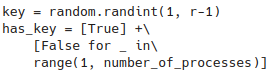
\includegraphics[width=0.70\linewidth]{Photos/HW4/key.png}
    \caption{
    مقداردهی اولیه‌ی کلید
    }
    \label{fig:my_label}
\end{figure}
کلید برای پروسه‌ی اول تولید می‌شود. آرایه‌ی
\texttt{has\_key}
نشان‌دهنده‌ی اینکه کدام پروسه‌ها کلید را می‌دانند، برای بقیه‌ی پروسه‌ها بجز این پروسه
\lr{False}
خواهد بود.\\
برای اینکه شبیه‌سازی بهتری از سیستم‌های سنکرون ارائه کنیم، با استفاده از تعدادی آرایه‌ی کمکی، مقادیر دور قبلی هر نود ذخیره شده و در پایان دور بعدی آپدیت می‌شود:
\begin{figure}[H]
    \centering
    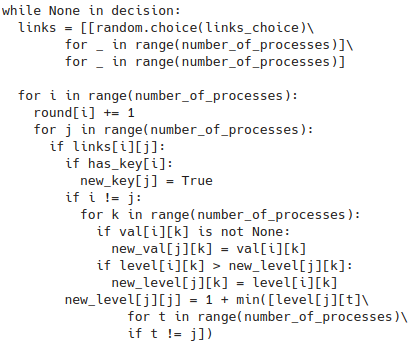
\includegraphics[width=0.99\linewidth]{Photos/HW4/loop.png}
    \caption{
    بدنه‌ی اصلی تکرار الگوریتم 
    }
    \label{fig:my_label}
\end{figure}
در اینجا آرایه‌هایی که نام آن‌ها با
\lr{new}
آغاز شده‌است در واقع نتیجه‌ی دور بعدی را نگه می‌دارند و تا اتمام اجرای حلقه، در هر مرحله مقادیر با استفاده از آن‌ها تغییر می‌کند.
\begin{figure}[H]
    \centering
    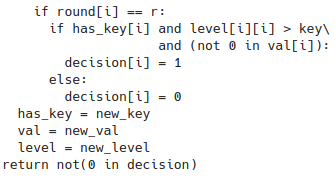
\includegraphics[width=0.80\linewidth]{Photos/HW4/finish.png}
    \caption{
    تصمیم‌گیری و پایان الگوریتم
    }
    \label{fig:my_label}
\end{figure}
تا وقتی که همه‌ی نودها تصمیم نگرفته‌اند، حلقه ادامه پیدا می‌کند. با توجه به احتمال از پیش مشخص شده، وضعیت سلامت لینک‌های ارتباطی برای این راند مشخص می‌شود.\\
در اینجا
\lr{i}
ارسال‌کننده و
\lr{j}
دریافت‌کننده فرض شده است.\\
اگر لینک ارتباطی سالم در نظر گرفته شود، با توجه به ساز و کار الگوریتم، پیام به نود مقصد می‌رسد و وضعیت بردارها آپدیت می‌شود. این کار تا جایی ادامه پیدا می‌کند که هیچ وضعیت نامعلومی در آرایه‌ی
\lr{decision}
وجود نداشته باشد. در نهایت با توجه به اینکه نظر همه‌ی نودها یک در نظر گرفته شده بود، تابع در صورتی که هیچ صفری در تصمیمات وجود نداشته باشد، یک برمی‌گرداند.
\begin{figure}[H]
    \centering
    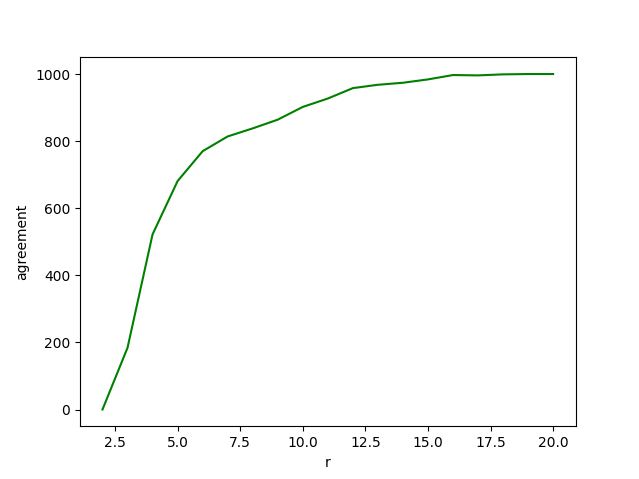
\includegraphics[width=0.99\linewidth]{Photos/HW4/one.png}
    \caption{
    توافق بر روی یک، بر حسب
    \lr{r}
    های مختلف
    }
    \label{fig:my_label}
\end{figure}
پیش‌تر صحبت شده بود که
$\dfrac{1}{r}$
حد مناسبی برای خطاست. با در نظر گرفتن احتمال
$\dfrac{1}{5}$
برای نرسیدن هر پیام، به نمودار زیر می‌رسیم:
\begin{figure}[H]
    \centering
    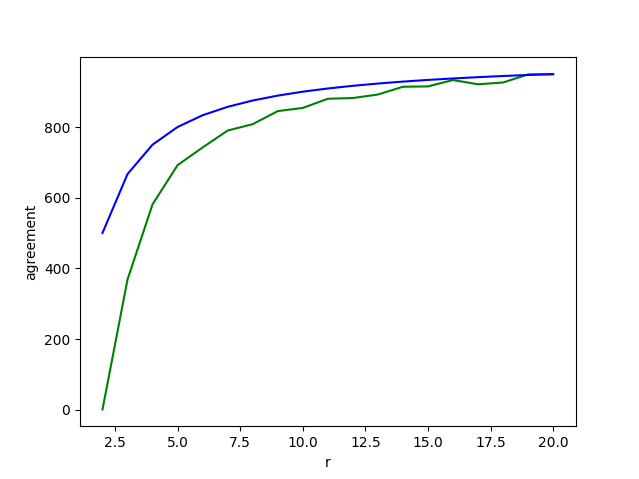
\includegraphics[width=0.99\linewidth]{Photos/HW4/one_per_r.png}
    \caption{
    مقایسه‌ی نتایج بدست آمده با نمودار خطای
    $\dfrac{1}{r}$
    که با رنگ آبی نشان داده شده است.
    }
    \label{fig:my_label}
\end{figure}
واضح است که هرچه دورهای اجرای الگوریتم بیشتر شود، درصد توافق‌ها نیز به ۱۰۰ نزدیک خواهد شد.\\
حال برای مثالی که در ابتدای گزارش ذکر شد (برای ۵ پروسه) با فرض اینکه همه‌ی نودها از ابتدا نظرشان یک باشد، با احتمال
$\dfrac{1}{10}$
برای از دست رفتن هر پیام، به میانگین موفقیت حدود ۹۷ درصد می‌رسیم که در شکل بعدی قابل مشاهده است.
\begin{figure}[H]
    \centering
    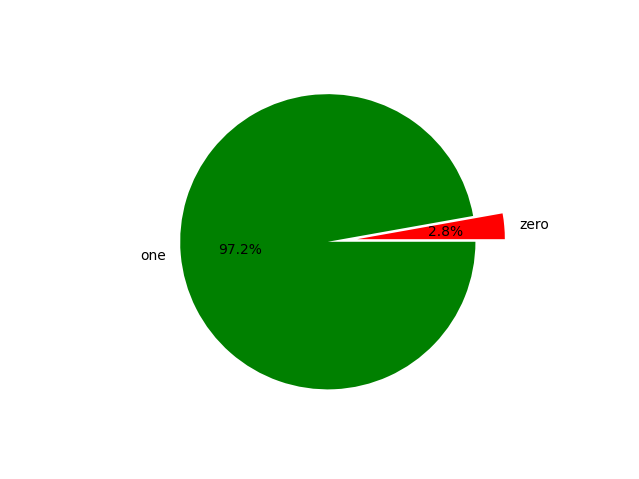
\includegraphics[width=0.99\linewidth]{Photos/HW4/percent.png}
    \caption{
    بخش سبزرنگ درصد توافق‌ها بر روی یک و بخش قرمزرنگ درصد توافق‌ها بر روی صفر را نشان می‌دهد.
    }
    \label{fig:my_label}
\end{figure}
تمامی نتایج مذکور از ۱۰۰۰ بار فراخوانی تابع حمله‌ی رندوم بدست آمدند.\\
با توجه به اینکه قطعه کدهای ترسیم نمودارها فاقد ارزش مثبت در جهت عملکرد الگوریتم بودند، از توضیح پیاده‌سازی آن‌ها صرف‌نظر شد.
\section*{بررسی شرایط سه‌گانه}
با توجه به شرط حلقه، این الگوریتم همواره خاتمه می‌یابد یعنی شرط
\lr{Termination}
برقرار است. همچنین اگر همه با صفر شروع کنند نتیجه‌ی نهایی الزاما صفر است و اگر احتمال از دست رفتن پیام‌ها صفر باشد، با توجه به اینکه گراف کامل است، نودها با شروع از یک، در پایان نیز بر روی یک توافق خواهند کرد و
\lr{Validity}
نیز برقرار است.\\
در مورد
\lr{Agreement}
نیز به طور مفصل در بخش قبلی توضیح داده شد.
\end{multicols}
\end{document}
